 
\section{Rezultatai}
\begin{figure}[p]
\centering
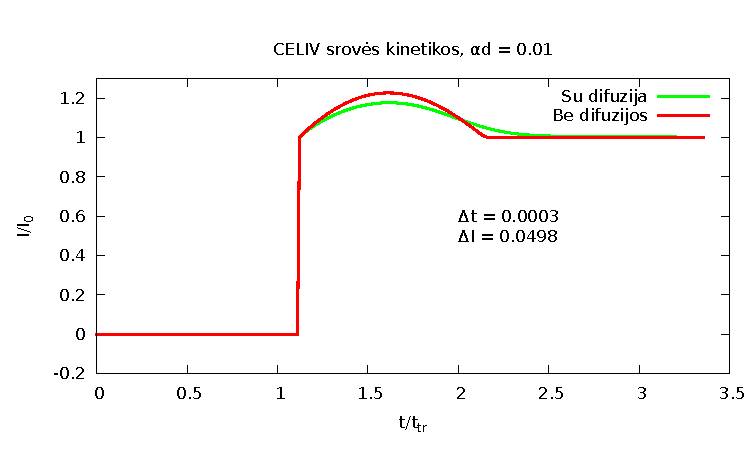
\includegraphics[width=\textwidth]{./media/pdf/ad001.pdf} 
\caption{Skirtumas tarp CELIV kinetikų esant difuzijai ir be jos tūrinės sugerties atveju}
\label{fig:001}
\end{figure}
\begin{figure}[p]
\centering
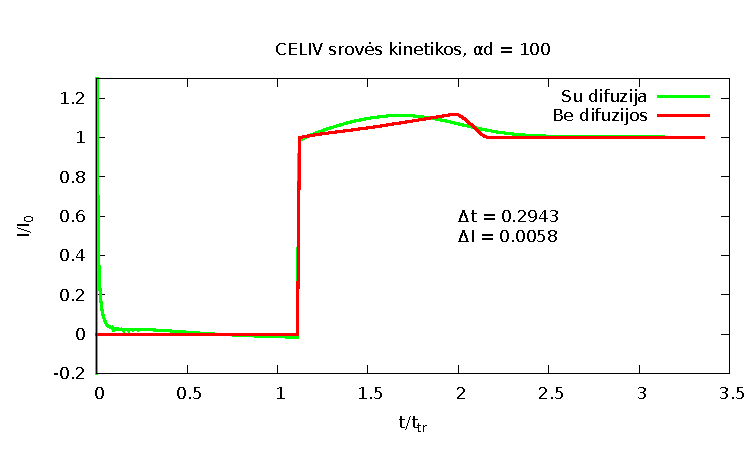
\includegraphics[width=\textwidth]{./media/pdf/ad100.pdf}  
\caption{Skirtumas tarp CELIV kinetikų esant difuzijai ir be jos paviršinės sugerties atveju}
\label{fig:100}
\end{figure}
\begin{figure}
  \centering
    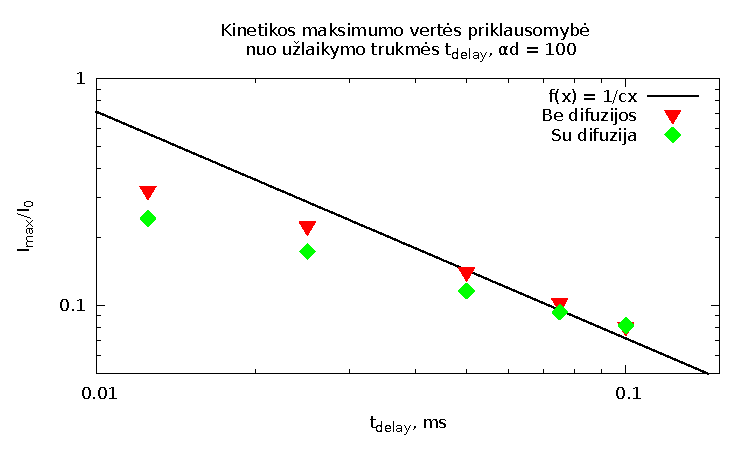
\includegraphics[width=\textwidth]{./media/pdf/ad100_recomb.pdf}
  \caption{Teorinių eksperimentų rekombinacijos nustatymui rezultatai}
  \label{fig:blockbuster}
\end{figure}
\begin{figure}
  \centering
    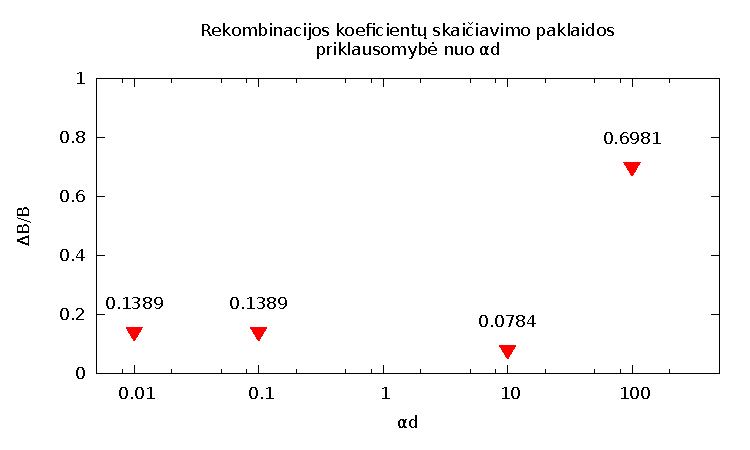
\includegraphics[width=\textwidth]{./media/pdf/beta.pdf}
  \caption{Paklaida tarp rekombinacijos koeficiento verčių suskaičiuotų įskaitant difuzija ir be jos, \(\Delta B = |B_{diff} - B_{nodiff}|\)}
  \label{fig:recomb}
\end{figure}
\begin{figure}
  \centering
    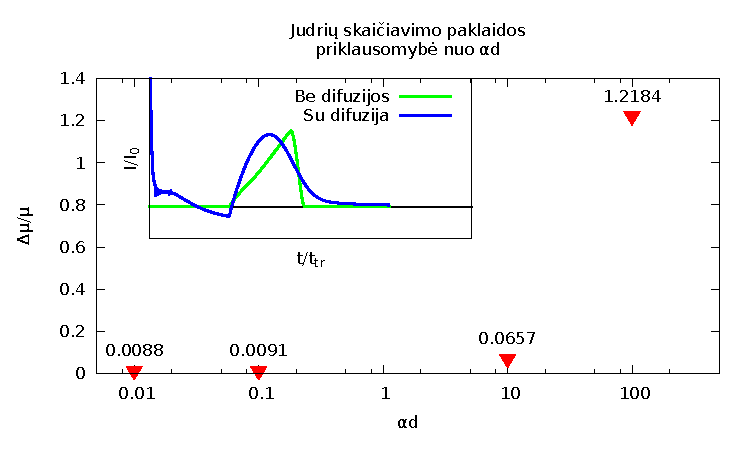
\includegraphics[width=\textwidth]{./media/pdf/mu.pdf}
  \caption{Paklaida tarp judrio verčių suskaičiuotų įskaitant difuziją ir be jos, \(\Delta \mu = |\mu_{diff} - \mu_{nodiff}|\)}
  \label{fig:mobility}
\end{figure}

Skaitmeniškai sumodeliuoti atskiri atvejai su difuzija ir be jos su skirtingais parametrais.

Patvirtinome, jog kinetikos maksimumas ir jo padėtis yra pakeičiami dėl difuzijos. Rezultatai pateikti \ref{fig:001} pav. ir \ref{fig:100} pav.
Akivaizdu, kad difuzija turi daug didesnę įtaką kai krūvininkai sugeneruoti paviršiuje, nes krūvininkų tankio gradientas prie paviršiaus yra didelis.

Photo-CELIV maksimumo padėtis leidžia nustatyti krūvininkų judrį pagal sąryšį:
\begin{equation}
\label{eq:judris}
\mu = K^2 \frac{2d^2}{At_{max}^2}
\end{equation}
Čia \(K\) - korekcijos koeficientas aptartas anksčiau paskelbtame darbe \cite{juška:155202}. Suskaičiavus \(\mu\) paklaidas esant skirtingiems sugerties profiliams (žr. \ref{fig:mobility} pav.) matome, jog difuzija kritinę įtaką turi matavimams, kurie atlikti esant stipriai paviršinei sugerčiai \(\alpha d = 100\). Šiuo atveju neįskaitant difuzijos srovė yra ribojama dėl krūvininkų sukuriamo elektrinio lauko. Jei įskaitoma difuzija -- srovė nėra ribojama. Dėl šio skirtumo negalima naudoti vienodų formulių judrio suskaičiavimui.

Pastaruoju metu dažnai rekombinacijos spartos matavimas atliekamas stebint kinetikos soties nuo intensyvumo reiškinį. Tačiau modeliavimo metu susidurta su sunkumais, kurie aprašyti priede \ref{app:rekombinacija}. Dėl to pasirinktas kitas rekombinacijos spartos matavimo būdas -- išmatuojant photo-CELIV kinetikos maksimumo vertės priklausomybės nuo \(t_{delay}\).
Iš šios priklausomybės galima nustatyti rekombinacijos tipą ir spartą.
Simuliavus rekombinacijos spartos eksperimentą su ir be difuzijos, gautos paklaidos pavaizduotos \ref{fig:recomb} pav. Matome, jog pasikeitus kinetikos pavidalui (esant paviršinei generacijai) rekombinacijos koeficiento paklaida viršija 50\%. Pagal \(\alpha d = 100\) teorinio eksperimento rezultatus (\ref{fig:blockbuster} pav.) matome, jog difuzija pakeičia rekombinacijos spartą. Pagal rezultatus, bandinyje vyksta bimolekulinė rekombinacija, taigi tipo nustatymui difuzija įtakos neturi.

Taip pat pastebėtas difuzinės srovės pikas matomas \ref{fig:100} pav. kairėje pusėje, ties koordinačių pradžia. Šio piko atsiradimas seka iš pasirinktų kraštinių sąlygų, tiksliau iš užtvarinių kontaktų: esant paviršinei fotogeneracijai dėl difuzijos atsiranda kryptingas krūvininkų judėjimas, nukreiptas nuo paviršiaus į bandinio vidų. Priklausomai nuo krūvininkų judrių srovė gali būti teigiama, neigiama, arba lygi nuliui, jei judriai lygūs ir krūviai neatsiskiria erdvėje. Kol kas photo-CELIV eksperimentuose toks pikas nebuvo stebimas, manoma, jog dėl krūvininkų atsiskyrimo mechanikos skirtumų. Modelyje priimta, kad nevyksta jokie papildomi krūvininkų atsiskyrimą užlaikantys reiškiniai ir fotonai iš karto generuoja atsiskyrusias poras. Tuo tarpu saulės elementuose vyksta daugiapakopis atsiskyrimas.

Nenumatytas rezultatas -- neigiama srovė atsirandanti dėl dreifo, difuzijos ir rekombinacijos tarpusavio sąveikos. Platesnis paaiškinimas priede \ref{app:video}. Šios srovės priežastis ir stebėjimo ribas planuojama tirti tolimesniuose tyrimuose.

\pagebreak
\section{Pagrindiniai rezultatai ir išvados}

\begin{itemize}

\item Photo-CELIV eksperimento metu, esant paviršinei sugerčiai \(\alpha d > 10\), privalu pasirinkti judrio skaičiavimo metodiką, pagal matomos kinetikos pavidalą.

\item Naudojant standartinę photo-CELIV formulę \eqref{eq:judris} gaunama paklaida tarp judrio verčių su difuzija ir be jos siekia 120\%.

\item Dėl difuzijos įskaitymo rekombinacijos tipas nepakinta, net ir esant paviršinei sugerčiai (\(\alpha d = 100\)).

\item Neatsižvelgus į difuzijos įtaką skaičiuojant rekombinacijos spartą, esant paviršinei sugerčiai \(\alpha d = 100\), galima padaryti paklaidą siekiančia 70\%.

\item Pastebėta atgalinė srovė tekanti esant paviršinei krūvininkų generacijai dar neįjungus CELIV įtampos signalo. Manome, jog ji nepastebėta eksperimente dėl mažos vertės arba ją slepia kiti efektai.

\end{itemize}


\pagebreak